\documentclass{beamer}

\usetheme{Hokie}
\usepackage{palatino}

\title{Graph Algorithms for  Visualizing High Dimensional Data}
\author{Abhinav Shankaranarayanan Venkataraman}
\institute{Universitat Politecnica de Catalunya (UPC), Barcelona}
\date{27 June 2016}

\graphicspath{{./}}
\DeclareGraphicsExtensions{.png}
\logo{
\includegraphics[height=0.5cm]{logo.png}}
\setbeamertemplate*{logo}

\begin{document}

\frame{\titlepage}

\section[Outline]{}
\frame{\tableofcontents}
\section*{LARCA}
\frame{
\frametitle{Project Research Group}
The project is done under the umbrella of LARCA(Laboratory
for Relational Algorithmics, Complexity and Learning)
  Project Directors :
  \begin{itemize}
  \item Prof. Ricard Gavalda Mestre
    \item Prof. Marta Arias Vicente
  \end{itemize}
}
\section{Introduction}
\subsection[What is a Community?]{Community Structure}

\frame
{
	\frametitle{An example slide}
	
	This is an example basic slide. It just has some text on it, no figures, tables, proofs, math, etc.  Note that Beamer lets have a 'long title' and a 'short title', used for sectioning and navigation. \cite{snapnets}
}

\frame
{
	\frametitle{Example Bullet List}

	This is an example of a bulleted list. Note that the bullets can be customized per the indent level.
	
	\begin{itemize}
	\item Hello, I am a bullet.
	\begin{itemize}
		\item This is a sub-bullet.
		\begin{itemize}
			\item This is a sub-sub-bullet.
		\end{itemize}
	\end{itemize}
	\vspace{\baselineskip}
	\item I am also a normal bullet..
	\end{itemize}
}

\section{Background}
\subsection[Few Theoretical Concepts]{Graphs}

\frame
{
	\frametitle{Graph}
	
}

\frame
{
	\frametitle{Example Bullet List}

	This is an example of a bulleted list. Note that the bullets can be customized per the indent level.
	
	\begin{itemize}
	\item Hello, I am a bullet.
	\begin{itemize}
		\item This is a sub-bullet.
		\begin{itemize}
			\item This is a sub-sub-bullet.
		\end{itemize}
	\end{itemize}
	\vspace{\baselineskip}
	\item I am also a normal bullet..
	\end{itemize}
}

\section{Louvain Community Detection Algorithm}

\frame
{
	\frametitle{Louvain Community detection Algorithm}

	This section has some examples of common slideshow elements.
}

\subsection{It's a table!!}

\frame
{
	\frametitle{Example Table}
	
	\begin{table}
	\centering
	\begin{tabular}{|c|c|c|} \hline \hline
	Restrained     & Swivel         & Telemetry      \\ \hline \hline
	$\sim$ 400bpm  & $\sim$ 380bpm  & $\sim$ 310 bpm \\
	$\sim$ 140mmHg & $\sim$ 120mmHg & $\sim$ 100mmHg \\ \hline \hline
	\end{tabular}
	\caption{Heart beat and blood pressure using different monitoring methods}
	\label{tbl:kramer}
	\end{table}
}

\subsection{HOW DO I DO MATH??}
\frame
{
	\frametitle{Example of a Theorem}
	It is easy to include mathematical theorems and such:
	\begin{theorem}
	The quick brown fox jumps over the lazy dog.
	\end{theorem}
}


\subsection{Everybody loves a good downsample.}
\frame
{
	\frametitle{Example Figure}
	
	\begin{figure}
	\centering
	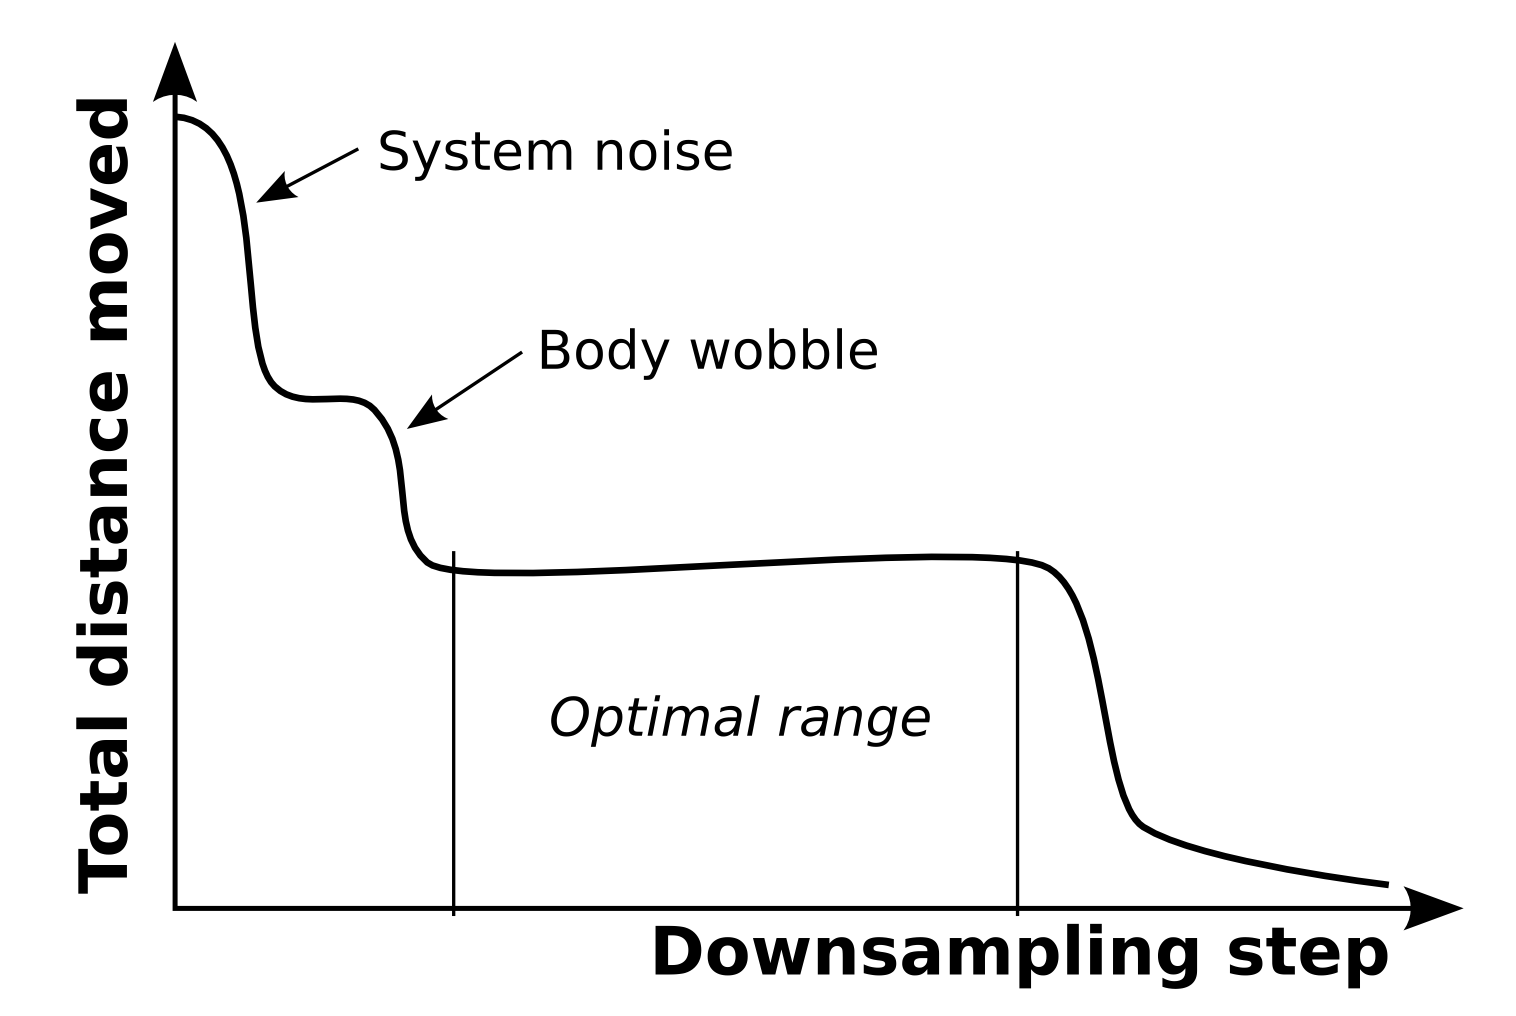
\includegraphics[width=5cm]{sample_rate.png}
	\caption{Our own test of downsampling}
	\label{fig:test_down_sampling}
	\end{figure}
}

\subsection{some numbers}
\frame
{
	\frametitle{Example Equation}

	\[8 / 4 = \frac{8}{4} = 8 \cdot \frac{1}{4} = 8 \cdot 4^{-1}\]
	
	\[\left( \begin{array}{cc}
	2 & 1 \\
	0 & 1 \\
	1 & 4 \\
	\end{array} \right)\]
}

\section{Conclusions}
\subsection{Personal Learning}


\subsection{Personal Learning}

\frame
{
	\frametitle{Personal Learning}
My interest towards data visualization has increase. I am interseted in 

}

\section{About}
\subsection{Last Slide}

\frame
{
	\frametitle{About}

	This slide show is mostly to demo the Hokie Beamer theme and see how it looks in various slideshow elements.  Some parts of the presentation are taken from Jean-Etienne Poirrier's example presentation, which can be found here:  \href{http://www.poirrier.be/~jean-etienne}{http://www.poirrier.be/~jean-etienne}.
	
	
\bibliographystyle{plain}
\bibliography{mybib}{}
}

\section{References}

\frame
{
	\frametitle{List of References that were used}

\bibliographystyle{plain}
\bibliography{mybib}{}
}
\section{Gracies}

\frame
{
	\frametitle{Thank you}
Thank you for all those who supported me throughout the project.\\
It was a Great time at Barcelona working with Prof.Ricard and Prof.Marta.
\bibliographystyle{plain}
\bibliography{mybib}{}
}

\end{document}
